\documentclass{beamer}
\usetheme{Madrid}
\usecolortheme{beaver}

\usepackage{graphicx, wrapfig, subcaption}
\usepackage{amsmath, amsfonts, amssymb, amsthm}
\usepackage{upgreek}
\usepackage{mathtools}
%\usepackage[skip=8pt]{parskip}
\usepackage{xcolor, hyperref}
%\usepackage{xspace}
\usepackage{xargs}
%\usepackage[label=\arabic*]{enumitem}
%\usepackage{booktabs}
\usepackage{tabularx}

\usepackage[
    backend=biber
]{biblatex}
\addbibresource{ref.bib}
\usepackage{appendix}

\usepackage{macros2}

\title{Sinusoidal Distribution}
\subtitle{A new flexible 4-parameter absolutely-continuous probability distribution}
\author{Baidurya Bhattacharyya\inst{1}}
\institute[ISI]{\inst{1} MD2403, M. Stat. 2nd Year\\ Indian Statistical Institute, Kolkata}
\date{\today}


\begin{document}
\maketitle

\section{Introduction}
\begin{frame}{The sinusoidal shape}
The sine function over $[0, \pi]$ has a nice `bell" shape indeed. Let us rescale the argument and deal with $\sin(\pi x)$ over $x \in [0,1]$.
\begin{itemize}
    \item But what about its powers -- $\sin^k(\pi x)$ as $k$ varies?
    \begin{figure}
        \centering
        
\includegraphics[width=0.5\linewidth]{presfig/p1-sinek}
    \end{figure}
    \item And what about powers of its argument -- $\sin(\pi x^s)$ as $s$ varies?
    \begin{figure}
        \centering
        
\includegraphics[width=0.5\linewidth]{presfig/p1-sines}
    \end{figure}
\end{itemize}
A first attempt at controlling ``peakedness" and ``inclination" intuitively! We can even combine both the operations to control them simultaneously!

\begin{enumerate} \item Hence the choice $\sin^k(\pi z^s)$ for the kernel! \end{enumerate}
\end{frame}

\begin{frame}{Other ``sine" distributions}
    \begin{table}[h]
        \centering
        \begin{tabular}{c|c}
            Work & Distribution \\
            \cite{gilbert1893moon} & \\
            \cite{sakthivel2021transmuted} & 
        \end{tabular}
        \caption{Caption}
        \label{tab:othersines}
    \end{table}
\end{frame}

\section{Sinusoidal Distribution}
\begin{frame}{Standard Distribution}
Notation: $Z \sim \Sinu(s,k)$
\begin{enumerate}
    \item Parameters: $s \ge 0$, $k\ge 0$
    \item Kernel: $\varsigma(z; s,k) := \sin^k(\pi z^s)$
    \item Normalizing constant $A(s,k) := \int_0^1 \sin^k(\pi t^s) \d t$
    \item PDF: $\psi(z; s,k) \equiv \frac{\varsigma(z; s,k)}{A(s,k)} = \frac{1}{A(s,k)} \sin^k(\pi z^s); \quad z \in [0,1]$
    \item $\Psi(z; s,k) = \int_0^z \psi(t; s,k) \d t \equiv \frac{A_z(s,k)}{A(s,k)}; \quad z\in[0,1]$ where $A_z(s,k)$ denotes the incomplete integral of the kernel
    
\end{enumerate}
\end{frame}

\begin{frame}{Plots}
   \begin{figure}
        \begin{subfigure}{0.45\textheight}
            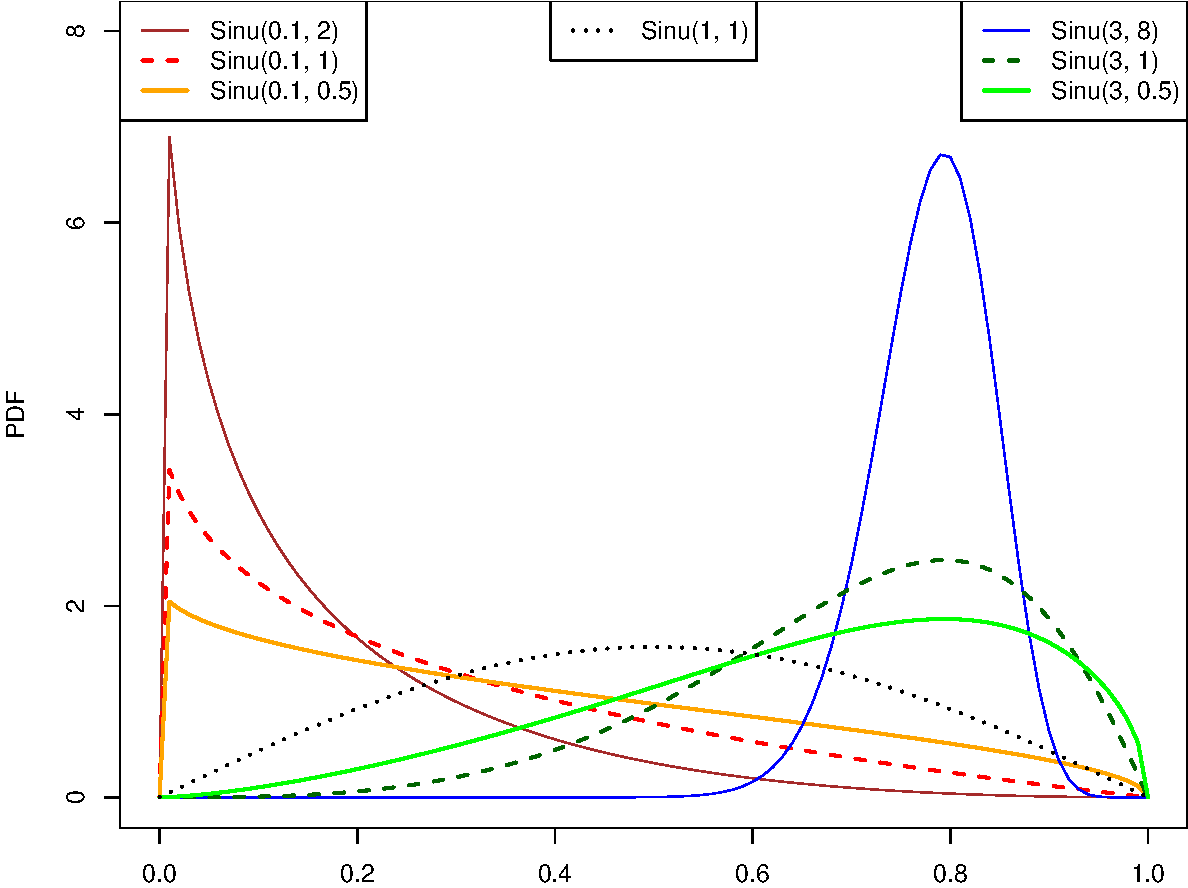
\includegraphics[width=\linewidth]{fig/2-pdf}
            \caption{PDFs}
        \end{subfigure}
        \begin{subfigure}{0.45\textheight}
            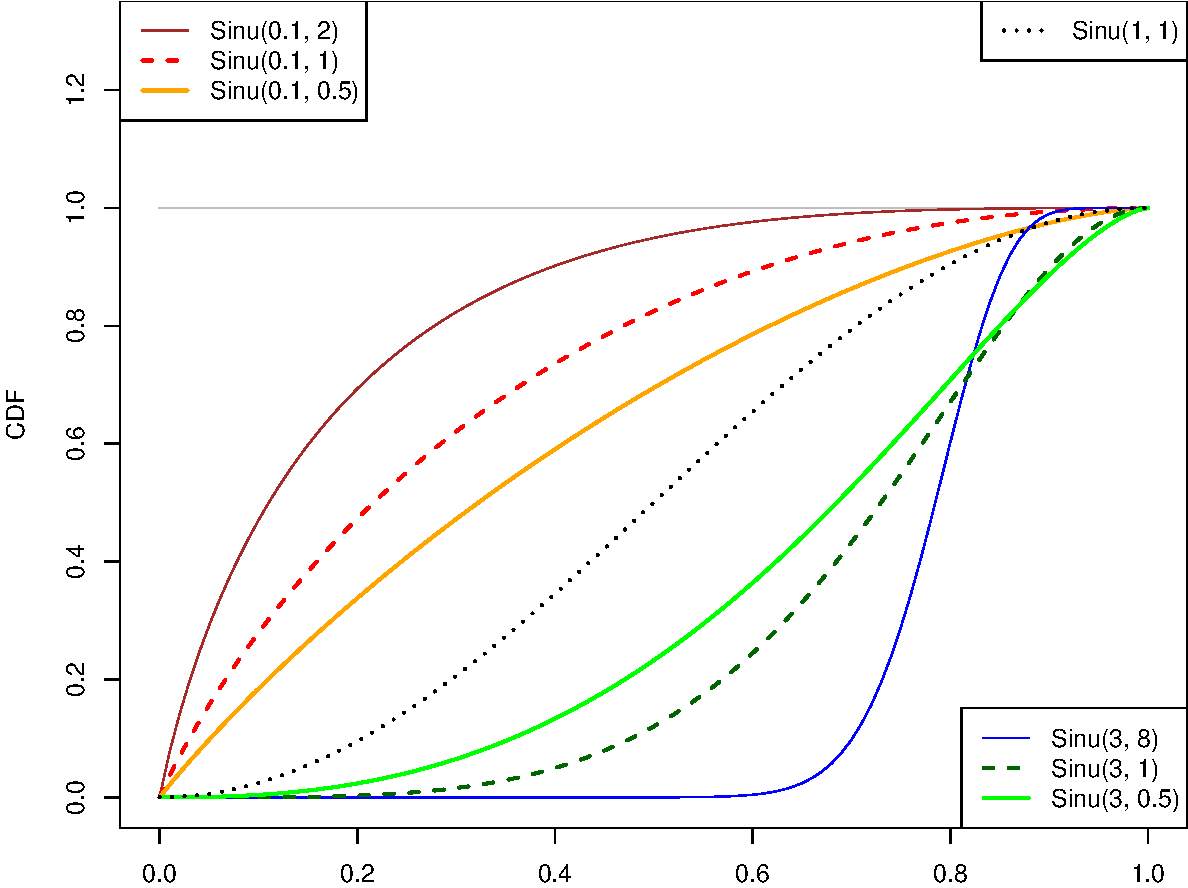
\includegraphics[width=\linewidth]{fig/2-cdf}
            \caption{CDFs}
        \end{subfigure}
        \begin{subfigure}{0.45\textheight}
            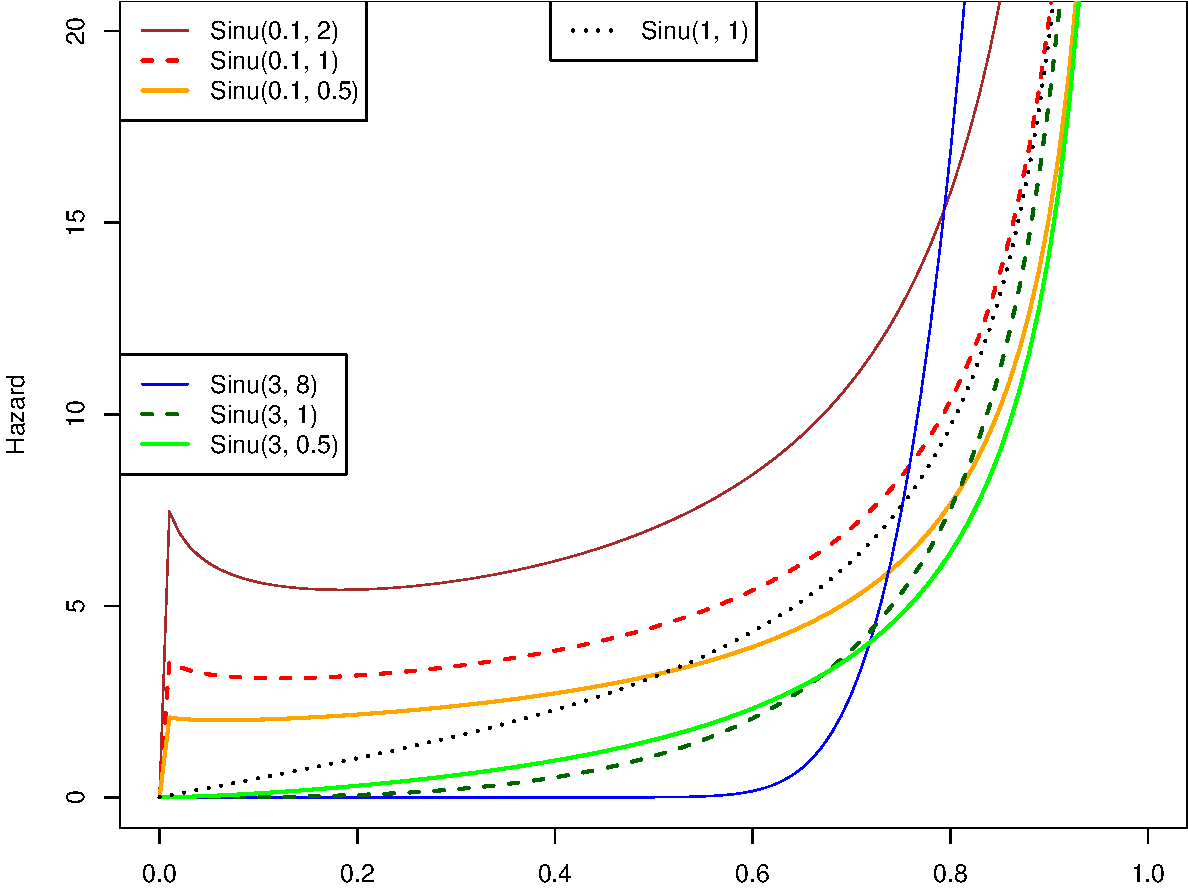
\includegraphics[width=\linewidth]{fig/2-hf}
            \caption{Hazard Functions}
        \end{subfigure}
        \begin{subfigure}{0.45\textheight}
            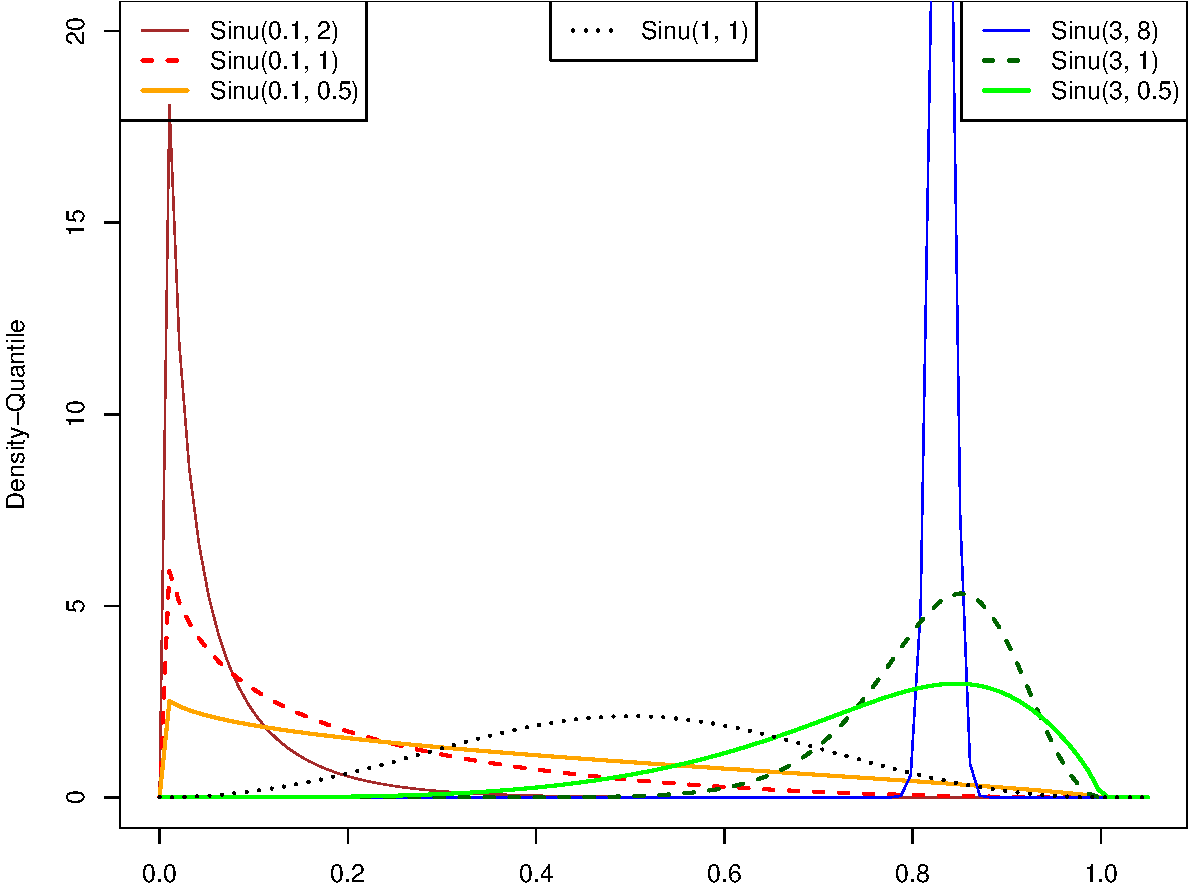
\includegraphics[width=\linewidth]{fig/2-dqf}
            \caption{DQFs}
        \end{subfigure}
        \caption{Shape plots of different \sindist s}\label{fig:shapeplots}
    \end{figure}
\end{frame}

\begin{frame}{Extensions}
\begin{enumerate}
    \item Location-Scale extension: $\psi(x; a,d,s,k) = {\frac 1 d} \psi \left( \frac{x-a}{d}; s,k \right);  \quad x \in [a, a+d]$ with parameters $a \in \RR, d \ge 0, s \ge 0, k\ge 0$
    \item Flipped extension: $ \pi'(x; a,d,s,k) = {\frac 1 d} \psi \left( \frac{a+d-x}{d}; s,k \right)$
\end{enumerate}
\end{frame}

\begin{frame}{Shape properties}
\begin{enumerate}
    \item Parameters: Location: $a \in \RR$, $d\ge0$, $s\ge0$, $k\ge0$
    \item Support $[a,a+d]$
    \item $s=1$: symmetric. Left and right tilts on respective sides of equality.
    \item Increasing $k$ first increases but then decreases kurtosis
    \item Mode: $2^{-1/s}$, Modal density: $1/A(s,k)$
\end{enumerate}
\end{frame}

\begin{frame}{Skewness-Kurtosis Interdependence on $s,k$}
\begin{figure}
    \begin{subfigure}{0.48\linewidth}
        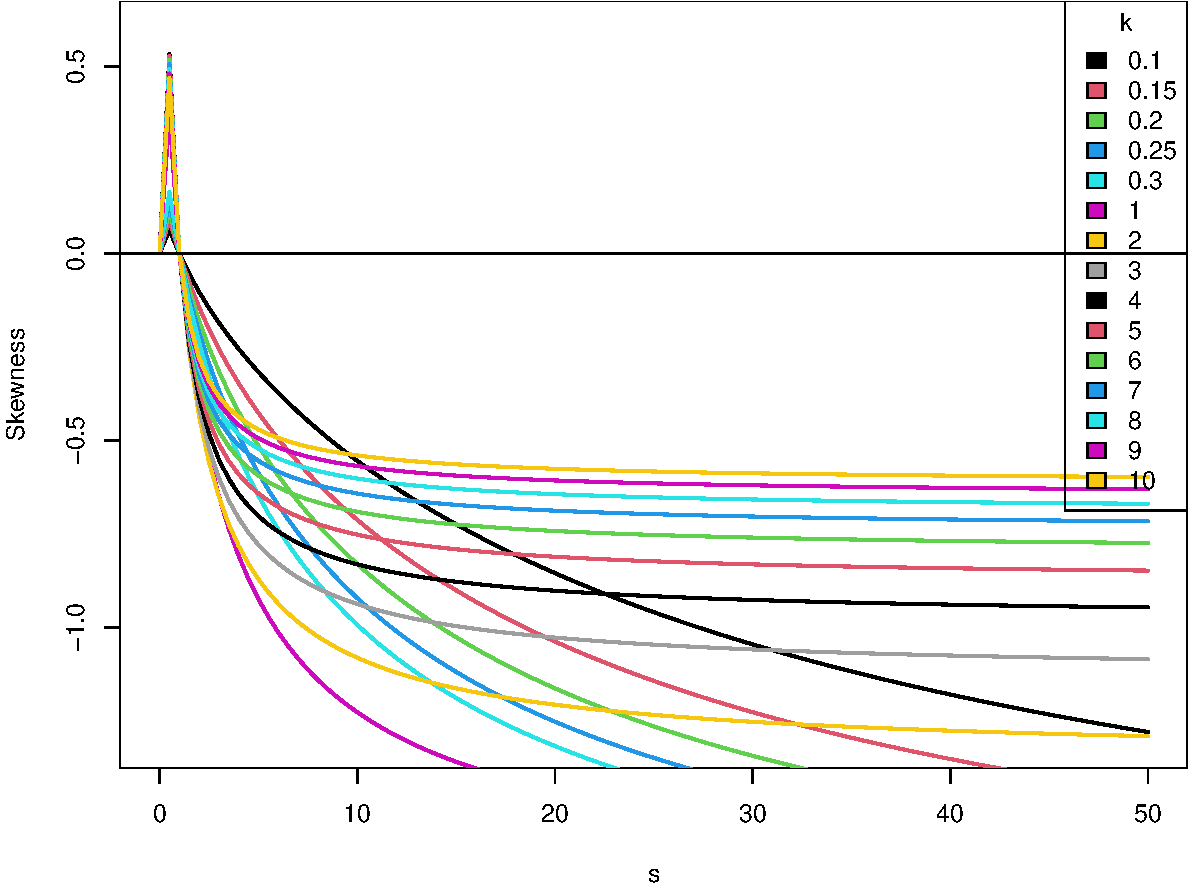
\includegraphics[width=\linewidth]{fig/2-skewvss}
        \caption{Skewness vs. $s$}
    \end{subfigure}
    \begin{subfigure}{0.48\linewidth}
        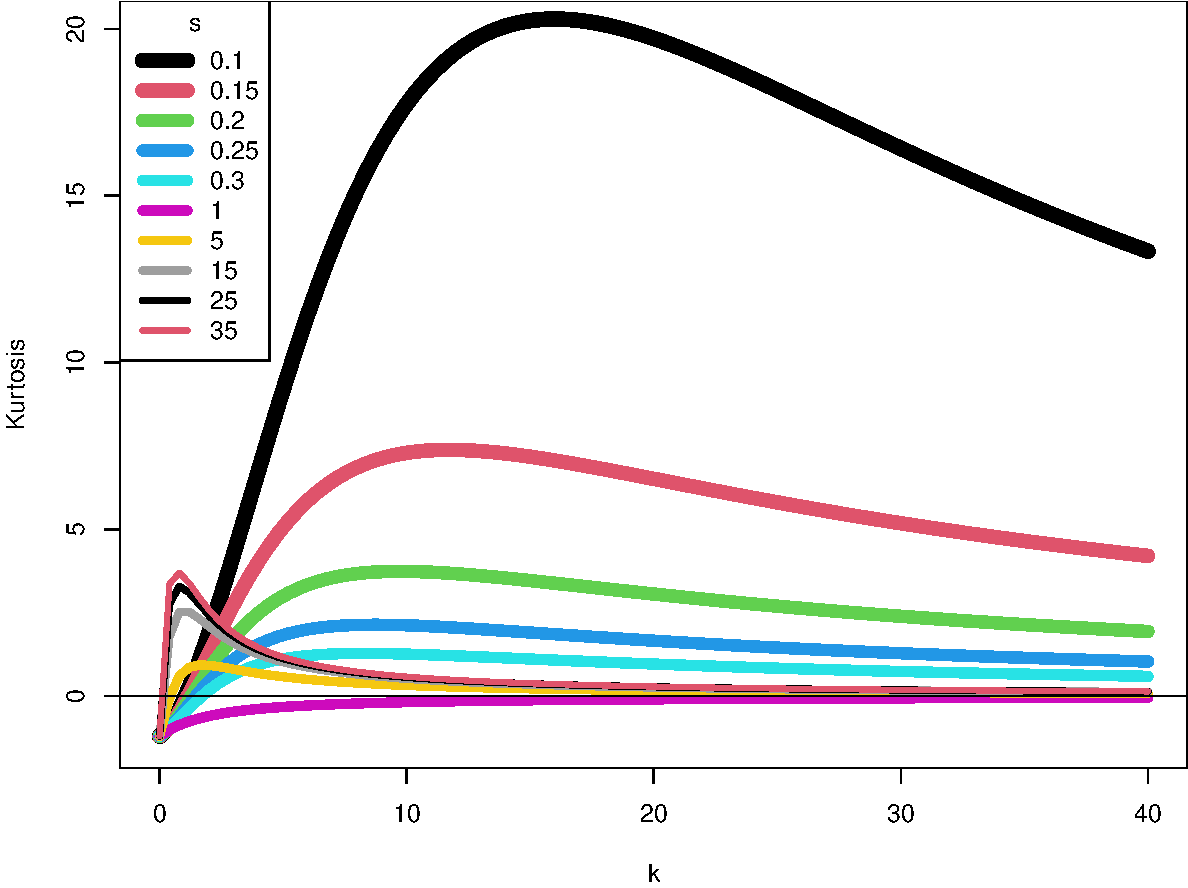
\includegraphics[width=\linewidth]{fig/2-kurtvsk}
        \caption{Kurtosis vs. $k$}
    \end{subfigure}
    \caption{$s$, $k$ jointly affect skewness \& kurtosis}\label{fig:skassoc}
\end{figure}
\end{frame}


\section{Mathematical Properties}
\begin{frame}[allowframebreaks]{Mathematical Properties}
\begin{enumerate}
    \item $\Sinu(s,k)$ distribution corresponds to the intensity of crater activity on the planetary surface given by the radial curve $r(z) = r_0 \exp\left(\int_0^{\pi z^s} \tan(t - \sin^{-1}\sin^k t) \d t\right)$
    \item $X_1, \dots, X_n \iidsim \Sinu(a,d,s,k)$ have joint density $f(x_1\dots x_n) = \frac{1}{A^n(s,k) 2^{nk} d^n } \left( \sum_{r_1=\pm1}\cdots \sum_{r_n = \pm 1} \left[\prod_{j=1}^n r_j\right] \cdot \exp\left[\sum_{j=0}^n \i \pi r_j \left(\frac{x_j -a}{d}\right)^s\right]  \right)^k$
    \item $\Sinu(a,d,s,k)$ is sub-Gaussian with parameter $d^2/4$
    \item The normalizing constant for the symmetric case is $A(1,k) = \frac{2^k}{\pi} \frac{\Gamma^2\left( \frac{k+1}{2} \right)}{\Gamma\left( k+1\right)} \equiv \frac{1}{\sqrt \pi} \frac{\Gamma\left(\frac{k+1}{2}\right)}{\Gamma\left(\frac{k}{2} + 1\right)}$
    \item 
\end{enumerate}
\end{frame}

%\section{Properties involving the HGF}

%\section{Fitting}

%\section{Future Applications}

\printbibliography


\end{document}